\documentclass[conference]{IEEEtran}
\IEEEoverridecommandlockouts
% The preceding line is only needed to identify funding in the first footnote. If that is unneeded, please comment it out.
\usepackage{cite}
\usepackage{amsmath,amssymb,amsfonts}
\usepackage{algorithmic}
\usepackage{graphicx}
\usepackage{url}
\usepackage[utf8]{inputenc}
\usepackage{textcomp}

\usepackage[english,ngerman,brazilian]{babel}
\def\BibTeX{{\rm B\kern-.05em{\sc i\kern-.025em b}\kern-.08em
    T\kern-.1667em\lower.7ex\hbox{E}\kern-.125emX}}
\begin{document}

\title{Projeto Demonstrativo 2 - Calibração de Câmeras}

\author{\IEEEauthorblockN{Frederico Guth (18/0081641)}
\IEEEauthorblockA{\textit{Tópicos em Sistemas de Computação, ,} \\
\textit{Turma TC - Visão Computacional (PPGI)}\\
\textit{Universidade de Brasília}\\
Brasília, Brasil\\
fredguth@fredguth.com}
}

\maketitle

\begin{abstract}
This document is a model and instructions for \LaTeX.
This and the IEEEtran.cls file define the components of your paper [title, text, heads, etc.]. *CRITICAL: Do Not Use Symbols, Special Characters, Footnotes, 
or Math in Paper Title or Abstract.
\end{abstract}

\begin{IEEEkeywords}
component, formatting, style, styling, insert
\end{IEEEkeywords}

\section{Introdução}
Uma câmera faz um mapeamento geométrico do mundo 3D para o plano de uma imagem 2D. Conhecendo seus parâmetros intrínsecos, como distância focal e distorção da lente, e extrínsecos, sua rotação e translação no sistema de coordenadas do mundo real, é possível estimar a posição 3D de um objeto a partir de sua imagem\cite{tese}. 

Isto possibilita diversas aplicações: por exemplo, a mensuração da altura de pessoas registradas em vídeos de camêras de segurança ou a estimativas de posições de atletas em campo, entre outras.

\subsection{Objetivos}
Os objetivos deste projeto são a aplicação prática da teoria de calibração de câmeras e o desenvolvimento de uma "régua visual", capaz de medir um objeto através da sua imagem.

Mais especificamente deseja-se que sejam desenvolvidos programas usando a biblioteca OpenCV capazes de:
\begin{enumerate}
\item medir um segmento de reta em imagens através de cliques de mouse;
\item realizar a calibração de uma câmera digital, armazenando os parâmetros intrísecos e os coeficientes de distorções em arquivos XML;
\item realizar a calibração de uma câmera digital a partir de diferentes distâncias da câmera, calculando os parâmetros extrínsecos da mesma e avaliando a diferença dos resultados;
\item medir um objeto através de sua imagem e comparar com suas dimensões reais;
\item analisar os resultados obtidos.
\end{enumerate}
\section{Revisão Teórica}

\subsection{Câmera Estenopeica com Coordenadas Homogêneas}

\begin{figure}[ht!]
\begin{center}
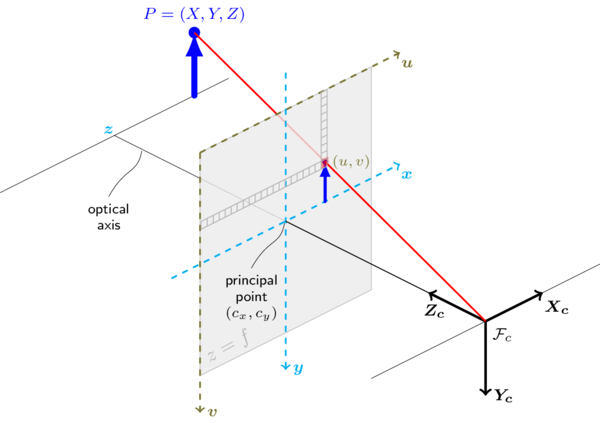
\includegraphics[width=0.75\columnwidth]{pinhole.png}
\caption{Modelo de Câmera Estenopeica\cite{docsopencv}}
\end{center}
\end{figure}

Se os pontos do mundo \(X\) e da imagem \(x\) são representados por coordenadas homogêneas, podemos expressar matematicamente a projeção da câmera como uma matriz\cite{tese}:

\begin{equation}\lambda  x = P  X\end{equation}

onde \(\lambda\) é um fator de escala e P é a matriz 3x4 de projeção, também chamada matriz de calibração.

P pode ser decomposto em duas entidades geométricas: os parâmetros intrísecos e extrísecos de calibração\cite{tese}
\begin{equation}
P = K [R | t]
\end{equation}
\begin{equation}
t = -R\widetilde{C}
\end{equation}
onde \(\widetilde{C}\) é a origem do sistema de coordenadas da câmera\cite{Hartley2004}.

Os parâmetros intrísecos de calibração descrevem a transformação entre a imagem ideal e a imagem em pixels
\begin{equation}
K = \begin{pmatrix} 
f & s & c_x \\
0 & \alpha f & c_y\\
0 & 0 & 1
\end{pmatrix}
\end{equation}
e os extrínsecos são a rotação \(R\) e translação \(t\) que transformam pontos no espaço do objeto para pontos no espaço da imagem e vice-versa\cite{tese}.

Como há 6 graus de liberdade nos parâmetros extrínsecos e 5 nos intrísecos, é necessário pelo menos 6 correspondências \({x_i \leftrightarrow X_i}\) do mesmo ponto no espaço da imagem e no espaço do objeto para obter P\cite{tese}. 

Dado que há um erro inerente nas medidas experimentais, para melhorar a qualidade da estimativa é preciso usar \(n > 6\) correspondências (como será visto em \ref{metodologia}, usaremos 48 pontos) e, assim, não há uma única matriz P que resolve esse sistema de equações. Precisamos, portanto, adicionar restrições para encontrar uma solução única.  

Um método comum é adicionar a restrição \(p_{34} = 0\)\cite{Hartley2004}, mas uma melhor abordagem\cite{tese} é:

\begin{equation}
\begin{aligned}
P = \min_{P'} \sum_{i}d(x_i, P'Xi)^2
\end{aligned}
\end{equation}
onde \(d(x_i, P'Xi) \) é a distância euclidiana entre o ponto observado e o estimado. 

\subsection{Distorções}

O modelo até aqui descrito descreve uma câmera ideal, mas as lentes das câmeras reais podem gerar distorções, que também são parâmetros intrínsecos que precisam ser considerados. 

A distorção radial causa uma curvatura no mapeamento.

(inserir imagem distorção)

A correção dessa distorção pode ser modelada da seguinte maneira\cite{docsopencv}: 

    \[x_{retificado} = x( 1 + k_1 r^2 + k_2 r^4 + k_3 r^6)\]
    \[y_{retificado} = y( 1 + k_1 r^2 + k_2 r^4 + k_3 r^6)\]

Outra distorção comum é a tangencial, que ocorre quando o plano da lente não está alinhado perfeitamente em paralelo ao plano da imagem. Para corrigir:


\[x_{retificado} = x + [ 2p_1xy + p_2(r^2+2x^2)] \]
\[y_{retificado} = y + [ p_1(r^2+ 2y^2)+ 2p_2xy] \]


Esses cinco parâmetros são conhecidos como coeficientes de distorção
\((k_1 \hspace{10pt} k_2 \hspace{10pt} p_1 \hspace{10pt} p_2 \hspace{10pt} k_3)\).

% [opencv-camera calibration]
\section{Metodologia}\label{metodologia}
O modelo da câmera e seus parâmetros foram descritos na seção de Revisão Teórica. Nesta seção, descreve-se como estimá-los experimentalmente.

\subsection{Materiais}
Foram utilizados:
\begin{itemize}
\item Uma tábua de compensado
\item Papel contact
\item Fita adesiva
\item Um padrão de calibração xadrez impresso em papel A4
\item Uma trena
\item Uma régua
\item Computador MacBook Pro (Retina, 13-inch, Early 2015), Processador Intel Core i5 2,7 GHz, 8GB de RAM
\item Python 3.6.3 :: Anaconda custom (64-bit)
\item OpenCV 3.4.0
\item sete programas em python especialmente desenvolvidos para o projeto. Todos estão disponíveis no repositório: \url{git@github.com:fredguth/unb-cv-3183.git}
\end{itemize}

\subsection{Preparação}
 \begin{enumerate}
 \item Imprime-se o padrão de calibração em folha A4 e o cola à tábua de compensado usando o Papel Contact.
 \item Com o programa \textit{requisito1.py}, abre-se uma imagem jpg e com cliques do mouse desenha-se um segmento de reta sobre a imagem entre o primeiro e o segundo clique, registrando-se a distância \(||p2 - p1||_2 \) na própria imagem aberta. 
 \end{enumerate}
\subsection{Obtenção dos parâmetros intrínsecos}
 \begin{enumerate}
  \item Executa-se o programa \textit{requisito2.capture.py} que abre um stream de vídeo e grava a imagem sempre que detecta os cantos dos quadrados no padrão de calibração de tabuleiro de xadrez. O programa pede o número do experimento e grava as imagens capturadas no diretório do mesmo.  Foram feitos 8 experimentos que geraram entre 25 e 70 imagens cada.
  \item Executa-se o programa \textit{requisito2.calibrate.py} para cada experimento. O programa detecta os cantos dos quadrados do padrão de calibração xadrez e refina essa deteção para obter os parâmetros intrínsecos K e os coeficientes de distorção. É importante mover o quadrado no campo de captura da câmera em diversas orientações e posições, em diferentes distâncias. Os parâmetros intrínsecos e coeficientes de distorção são automaticamente armazenados em arquivos xml nos diretórios dos respectivos experimentos.
\item Dado que já temos os coeficientes de distorção, com o programa \textit{requisito2.measure.py} retificamos as imagens da câmera e permitimos medir distâncias na imagem retificada em pixels. 
\item Após todos os experimentos executados, executa-se o programa \textit{requisito2.analyse.py} que gera a média e o desvio parão dos parâmetros intrísecos, salvando-os no diretório /textit{./exp-0/}.
\end{enumerate}
\subsection{Obtenção dos parâmetros extrínsecos}
\begin{enumerate}
\item Executa-se o programa \textit{requisito3.py}, que computa a correspondencia entre pontos da imagem e do espaço do objeto, atribuindo como origem do sistema de coordenadas do mundo, o ponto de intersecção do canto superior esquerdo do tabuleiro e através da função \textit{solvePnP} da OpenCV\cite{OpenCV}, obtem os parâmetros extrínsecos R e t. 
\item Quando o programa pede o número do experimento, escolhe-se \(0\), uma vez que queremos usar os parâmetros intrísecos médios, medidos na etapa anterior.

\item Deixa-se a câmera em um ponto marcado pela fita adesiva, tentando colocá-la ortogonal ao plano da sua base. 
\item Com a câmera posicionada, posiciona-se o tabuleiro na distância mais próximo possível da câmera em que o padrão de calibração tem seus cantos detectados (os cantos ficam marcados com pontos coloridos no \textit{stream} da câmera), marcando com a fita adesiva este ponto como \(d_{min}\). 
\item Repete-se o passo anterior, tentando encontrar a distância mais afastada da câmera em que os cantos do padrão de calibração ainda são detectáveis. Marca-se este ponto com fita adesiva como \(d_{max}\); e um ponto intermediário entre \(d_{min}\) e \(d_{max}\), que chamamos \(d_{med}\).
\item Medimos a distância da câmera à origem do padrão de calibração usando a trena. Para cada distância, obtemos três vezes os valores de R e t.
\item Com todos os pontos marcados e a câmera posicionada, acionamos o modo de captura apertando a tecla \textit{espaço}
\item Leva-se o tabuleiro de xadrez para \(d_{min}\) e após algumas capturas (identificação do padrão xadrez na imagem \textit{stream} da câmera), apertamos a tecla \textit{espaço} novamente para sair do modo captura.
\item Repete-se os últimos dois passos para as distâncias \(d_{med}\) e \(d_{med}\). As imagens captadas com as respectivas distâncias medidas são gravadas no diretório do experimento selecionado (no caso, \textit{./exp-0/}). 
\end{enumerate}
\subsection{Obtenção da altura de um objeto através da sua imagem}
Com os parâmetros intrínsecos e extrínsecos,  é possível medir um objeto no mundo real a partir da sua imagem. Neste projeto, entretanto, não se obteve êxito em desenvolver essa funcionalidade no programa \textit{requisito4.py}

\section{Resultados}
\subsection{Medição em pixels de segmentos de imagens}
\subsection{Obtenção dos parâmetros intrínsecos}
\subsection{Obtenção dos parâmetros extrínsecos}

\section{Discussão e Conclusões}
% \begin{table}[htbp]
% \caption{Table Type Styles}
% \begin{center}
% \begin{tabular}{|c|c|c|c|}
% \hline
% \textbf{Table}&\multicolumn{3}{|c|}{\textbf{Table Column Head}} \\
% \cline{2-4} 
% \textbf{Head} & \textbf{\textit{Table column subhead}}& \textbf{\textit{Subhead}}& \textbf{\textit{Subhead}} \\
% \hline
% copy& More table copy$^{\mathrm{a}}$& &  \\
% \hline
% \multicolumn{4}{l}{$^{\mathrm{a}}$Sample of a Table footnote.}
% \end{tabular}
% \label{tab1}
% \end{center}
% \end{table}

% \begin{figure}[htbp]
% \centerline{
\includegraphics{fig.jpg}}
% \caption{Example of a figure caption.}
% \label{fig}
% \end{figure}

\selectlanguage{brazilian}
\bibliographystyle{IEEEtran}
\bibliography{references}

\end{document}
